\documentclass[a4paper,11pt]{article}
\usepackage[T1]{fontenc}      % codifica dei font
\usepackage[utf8]{inputenc}
\usepackage[italian]{babel}
\usepackage{lipsum}
\usepackage{comment}
\usepackage{url}
\usepackage{amsfonts}
\usepackage{graphicx}
\begin{document}
% lettere accentate da tastiera
% lingua del documento
% genera testo fittizio
% per scrivere gli indirizzi Internet
\author{Linpeng Zhang}
\title{Tutorato AFL}
\maketitle
\begin{abstract}
    Per errori/dubbi/problemi: linpeng.zhang@studenti.unipd.it.
     \\Note: la lezione del 15 non ci sarà. Verrà recuperata la settimana successiva (verrete avvisati su Facebook e Telegram)
\end{abstract}
\tableofcontents
\section{Lez8}
\subsection{Esercizi}
\begin{enumerate}
    \item  Convertire in PDA la CGG seguente:\\
    \begin{minipage}{\linewidth}
       $S \rightarrow 0S1\ |\ A$\\
        $A \rightarrow 1A0\ |\ S\ |\ \epsilon$\\
   \end{minipage}
   \item  Convertire in PDA la CFG seguente:\\
   \begin{minipage}{\linewidth}
    $S \rightarrow aAA$\\
       $A \rightarrow aS\ |\ bS\ |\ a$\\
  \end{minipage}
   \item  Convertire in CFG il PDA seguente:\\
   \begin{minipage}{\linewidth}
       $ \delta (q,1,Z) = \{(q, XZ)\}$\\
       $ \delta (q,1,X) = \{(q, XX)\}$\\
       $ \delta (q,0,X) = \{(p, X)\}$\\
       $ \delta (q,\epsilon ,X) = \{(q, \epsilon )\}$\\
       $ \delta (p,1,X) = \{(p, \epsilon )\}$\\
       $ \delta (p,0,Z) = \{(q, Z)\}$\\
  \end{minipage}
  \item  Convertire in CFG il PDA seguente:\\
  \begin{minipage}{\linewidth}
      $ \delta (q,1,Z) = \{(q, 1Z)\}$\\
      $ \delta (q,0,Z) = \{(q, 0Z)\}$\\
      $ \delta (q,0,1) = \{(q, \epsilon)\}$\\
      $ \delta (q,1,0) = \{(q, \epsilon )\}$\\
      $ \delta (q,1,1) = \{(q, 11 )\}$\\
      $ \delta (q,0,0) = \{(q,00 )\}$\\
      $ \delta (q, \epsilon, Z) = \{(q, \epsilon)\}$\\
 \end{minipage}   
 \item Definire una CFG per $L=\{ a^ib^jc^k\ |\ i=2j $oppure $j=2k, i,j,j\geq 0\}$. Dimostrarne la correttezza. Convertirlo in PDA.
\end{enumerate}
\subsection{Soluzioni}
\begin{enumerate}
    \item \begin{minipage}{\linewidth}
        $\delta (q, \epsilon, S) = \{(q,0S1), (q,A)\}$\\
        $\delta (q, \epsilon, A) = \{(q,1A0), (q,S), (q, \epsilon)\}$\\
        $\delta (q, 0, 0) = \{(q,\epsilon)\}$\\
        $\delta (q, 1, 1) = \{(q,\epsilon)\}$\\
    \end{minipage}
    \item \begin{minipage}{\linewidth}
        $\delta (q, \epsilon, S) = \{(q,aAA)\}$\\
        $\delta (q, \epsilon, A) = \{(q, aS, (q,bS), (q, a)\}$\\
        $\delta (q, a,a) = \{(q,\epsilon)\}$\\
        $\delta (q, b,b) = \{(q,\epsilon)\}$\\
    \end{minipage}
    \begin{minipage}{\linewidth}
        $S \rightarrow [qZp]\ |\ [qZq]$\\
        $(1) [qZq] \rightarrow 1[qXp][pZq]\ | 1[qXq][qZq]$\\
        $(1) [qZp] \rightarrow 1[qXq][qZp] | 1[qXp][pZp]$\\
        $(2) [qXq] \rightarrow 1[qXq][qXq] | 1[qXp][pXq]$\\
        $(2) [qXp] \rightarrow 1[qXq][qXp] | 1[qXp][pXp]$\\
        $(3) [qXq] \rightarrow 0[pXq]$\\
        $(3) [qXp] \rightarrow 0[pXp]$\\
        $(4) [qXq] \rightarrow \epsilon$\\
        $(5) [pXp] \rightarrow 1$\\
        $(6) [pZq] \rightarrow 0[qZq]$\\
        $(6) [pZp] \rightarrow 0[qZp]$\\
      \end{minipage}
      \item \begin{minipage}{\linewidth}
        $S \rightarrow [qZq]$\\
        $(1) [qZq] \rightarrow 1[q1q][qZq]$\\
        $(2) [qZq] \rightarrow 0[q0q][qZq]$\\
        $(3) [q1q] \rightarrow 0$\\
        $(4) [q0q] \rightarrow 1$\\
        $(5) [q1q] \rightarrow 1[q1q][q1q]$\\
        $(6) [q0q] \rightarrow 0[q0q][q0q]$\\
        $(7) [qZq] \rightarrow \epsilon$\\
      \end{minipage}
      Naturalmente si possono scrivere le produzioni in modo più compatto.
       \item Una grammatica è:
       \begin{itemize}
       \item $S \Rightarrow TC | AP$
    \item $A \Rightarrow aA | \epsilon$
\item $C \Rightarrow cC | \epsilon$
\item $T \Rightarrow aaTb | \epsilon$
\item $P \Rightarrow bbPc | \epsilon $
       \end{itemize}
       Poiché si utilizzano più simboli, si deve (in genere) dimostrare la correttezza dei simboli annidati. In particolare, è banale dimostrare che A e C generino linguaggi di soli a e c.\\
       Successivamente si dimostra che $L(T)=\{a^ib^j \ |\ i=2j, \ i,j\geq 0 \}$ e $L(P)=\{b^jc^k \ |\ j=2k, \ j,k\geq 0 \}$. A questo punto è banale dimostrare la tesi di partenza.\\
       Applicando la conversione vista a lezione si ottiene:\\
    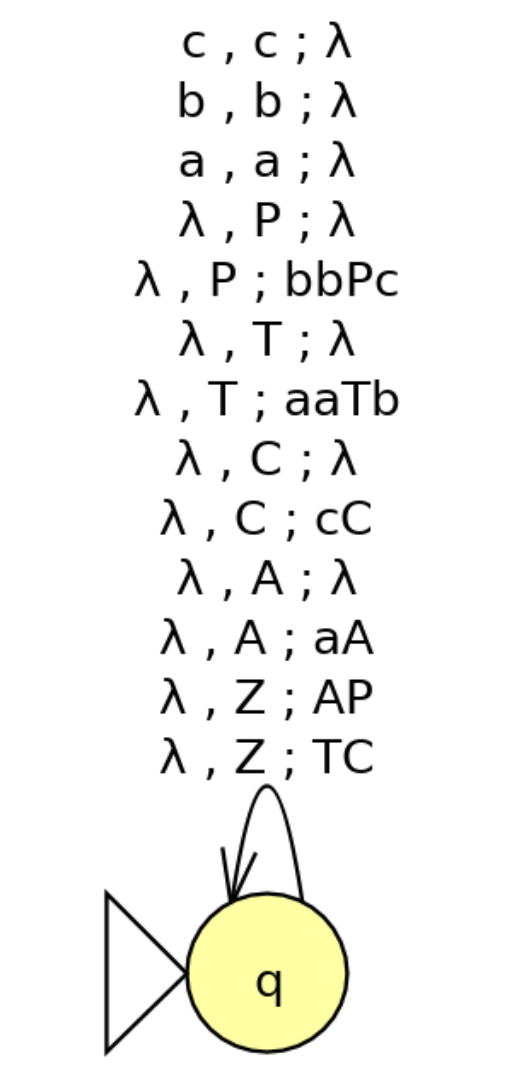
\includegraphics[scale=0.5]{Lez8solLast.png}
      %   \item si può dimostrare che A genera $L_A=\{a^nb^m|n=m+1$ oppure $n=m$ con $n>0,m\geq 0\}$, B genera $L_B=\{a^nb^m|m=n+1$ oppure $n=m$ con $m>0,n\geq 0\}$. Dalle due asserzioni precedenti si dimostra che S genera $L_S=\{a^nb^m|n=m+1$ oppure $n=m$ con $n,m>0\}$: infatti S produce le stringhe che produce B con una a all'inizio, e la correttezza segue dalla definizione.\\
   %  Un automa a pila che accetta tale linguaggio è:\\
  %  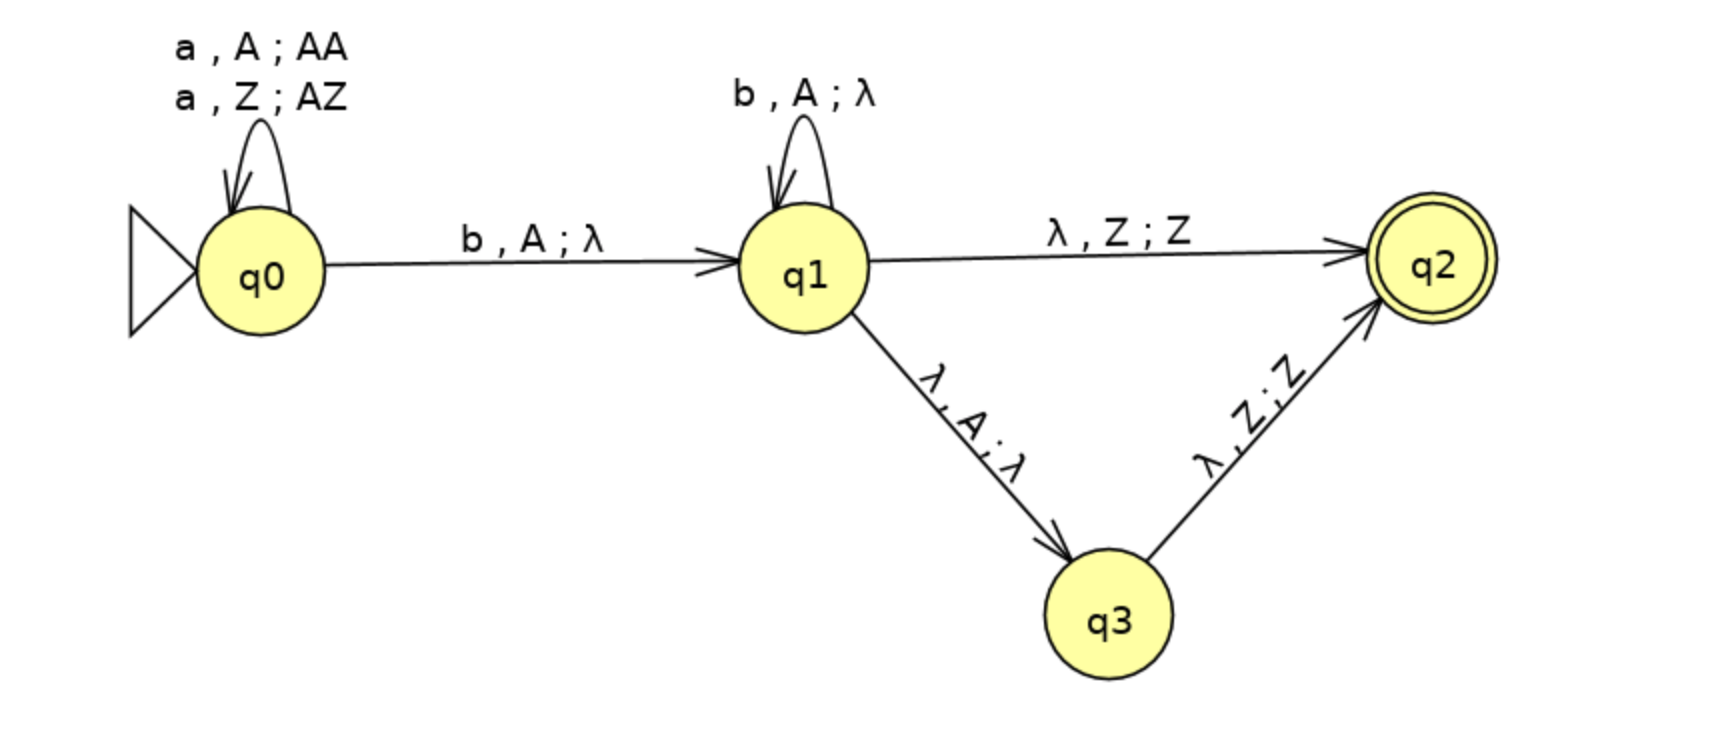
\includegraphics[scale=0.5]{Lez7sol6.png}
\end{enumerate}

\begin{comment}
       \item Sia data la CFG:\\
     \begin{minipage}{\linewidth}
        \centering $S \rightarrow aB$\\
        \centering $B \rightarrow Ab\ |\ b$\\
        \centering $A \rightarrow aB\ |\ a$\\
    \end{minipage}
    \\Dire: linguaggio accettato e definire un automa che accetti tale linguaggio.
\end{comment}
    % Bibliografia
    %\begin{thebibliography}{9}
        %  Alcune soluzio
    %\end{thebibliography}
    \end{document}